\documentclass[conference,11pt]{IEEEtran}
\usepackage{url}
\usepackage{ulem}
\usepackage{amssymb}
\usepackage{amsmath}
\usepackage{amsthm}
\usepackage{eurosym}
\usepackage{graphicx}
\graphicspath{{img/}}


\begin{document}

\title{Example Paper for MSE and MSSF}

\author{\IEEEauthorblockN{Charles Paulet}
\IEEEauthorblockA{ID: 18103197}
\and
\IEEEauthorblockN{John Watson}
\IEEEauthorblockA{ID: 87654321}
\and
\IEEEauthorblockN{James Moriarty}
\IEEEauthorblockA{ID: 87651234}}

\maketitle

\begin{abstract}
This is the report of the first ca645 assignment. Our task is to research and
implement a phishing URL classifier and to write a paper detailing your approach
and findings. This is the paper.
\end{abstract}

\section{Introduction}
In this document, we will describe the goals of the project, how we achieved
them, what difficulties we encountered and some suggestions for improvement.

\section{The goals of the project}
As previously written, the main goal is to research and implement a phishing URL
classifier. The research step is of course necessary for the implementation one.
We had some vague notions about machine learning but not as much as required by
this project. In fact, we had only theoretical knowledge of the field, it was
time for us to have a bit of practice. This project will also allow us to
conduct an assignment as a pseudo-real research work.

\section{Past experience in ML}
We had a few notions of machine learning. Let's sum it up. Charles had some fun
recently discovering multivariate statistics (PCA, LDA, \ldots) but nothing that
revelant nor very handy for this task. Even if it's closely related. Pierre
\ldots and Garçon gentil \ldots

\section{Our implementation}
For our implementation, we choose to used Python as a language not because of
its speed, memory consumption or runtime errors but because it was easy and fast
for us to script and quickly test models while enjoying many machine learning
frameworks. We decided to use scikit-learn because \sout{it is Français} of its
exhaustive documentation and its integration with other libraries like numpy,
pandas and matplotlib. We indeed relied on those to manipulate and display data.
From a technical point of view, we worked in test driven development especially
while working on features to ensure a dependancy-less and long-lasting code but
also to unitary test feature code and anticipate various kind of failure (some
due to Python runtime politics (mostly dynamic typing and exceptions)). To
ensure that the code will remain consistent and readable, we used pycodestyle, a
PEP-8 compliant linter. We used Git as a version control system and Gitlab
issues to discuss on the project.

\subsection{Gathering data}
We have a python package data that is responsible for gathering, saving and
loading data.

\subsection{Adding features}
We began to add two simple features before having the whole loop. We such began
with the length (as advised) and the subdomain count features.

\subsection{Features}
We will describe some of our features and the reason the they might be
interesting. Of course, we should limit strong preconceptions among their
ability to classify properly URLs. We tried to find features that have the most
unique characteristics and such the greatest fingerprinting capabilities,
whether it be for safe or unsafe URLs.

\subsubsection{length}
Length may be a useful metric, shortest domain names are usually the most
expensive, unless for new gTLDs.

\subsubsection{subdomains}
We can link an excessive amount of URLs to a particular domain thanks to the
subdomain diversity. Subdomains are cheap to set up and manipulate. They can be
used in a funny way with domain name (e.g. pay.pal.com ) which may lead to
target misinterpretation.

\subsubsection{TLD usage}
Old domain names can not / generally not use new gTLDs. The .com popularity is
nearly 50\% whereas the new .dev is still less than 1\%. \cite{tld-stats} There
is a large gap that might feed our model properly.

\subsubsection{days since registration of the domain}
Here we have to use network I/O which is pretty slow, but we think the nature of
the data worth it. We think that unsafe domains are newly registered (to remain
stealh or because older one had been detected).

\subsubsection{is ascii}
We are checking if the url charset can be restricted to ascii only. If not, it
permits mono-letter homograph attack because homographs aren't bound to the
ascii charset.

\subsubsection{russian TLD}
Adding the .ru russian TLD recognition as a feature surprisingly increased the
model, what came up as a joke remained as an asset.

\subsection{Visualization}
Visualization of data is a very important step on a data analysis approach. In
our case, it helped us in feature selection (quality over quantity) and in model
validation. We used two visualization tools in particular for feature selection:

\subsubsection{Scatter matrix}
The scatter matrix allows us to visualize the relationship between two
variables. It's an estimation of a covariance matrix. The figure
\ref{scatter-matrix-interpretation} shows how we should interpret the contents
of such a matrix. The figure \ref{scatter-matrix-right} is an exemple of perfect
correlation between two variables (which are the same for the sake of the
example). We are aiming for positive or negative linear relation between blue
and red points. The more the line is balanced (diagonal in the square), the more
strong the relation between the variables is. Scatter matrix is also a way to
reveal cluster of points which can orientate us in the model of classification
to be used and its parameters.

\begin{figure}[!t]
  \centering
  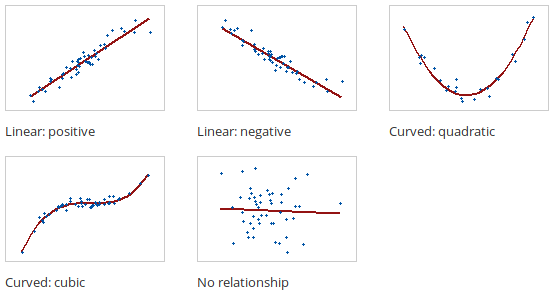
\includegraphics[width=\linewidth]{scatter_matrix_interpretation}
  \caption{Plots interpretation}
  \label{scatter-matrix-interpretation}
  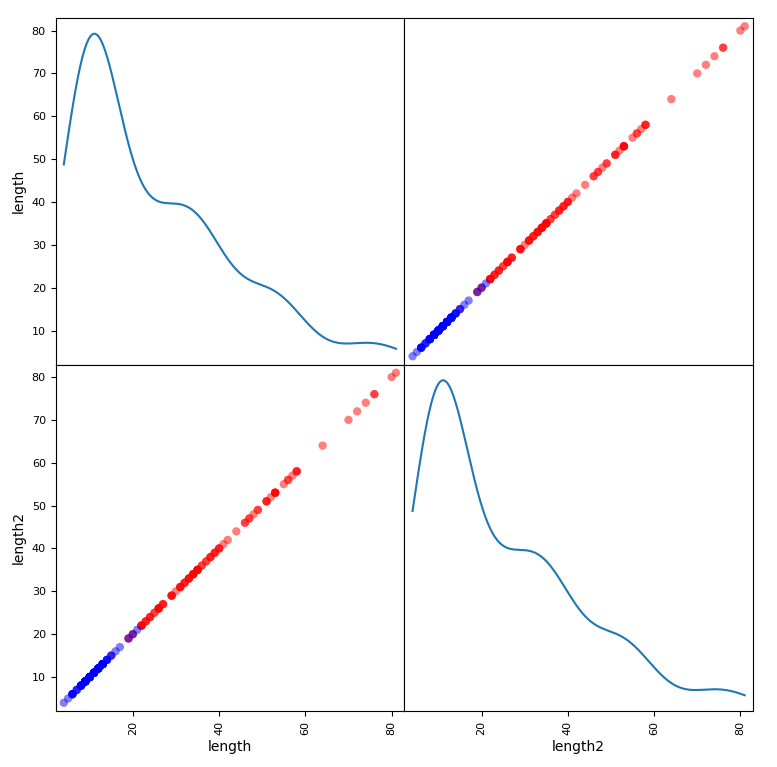
\includegraphics[width=\linewidth]{scatter_matrix_lengths_correlation_right}
  \caption{Strongest relation possible}
  \label{scatter-matrix-right}
\end{figure}

\subsubsection{Correlation matrix}
The correlation matrix is another tool to visualize the relationship between two
variables. For that one, we linked all the variables in a triangle where the
color hue of variable intersections expresses the correlation coefficient for
the two variables intersected. The figure \ref{correlation-matrix} is an example
some of our features. As expected, we can see a strong correlation between the
number of subdomains and the length of the URL.

\begin{figure}[!t]
  \centering
  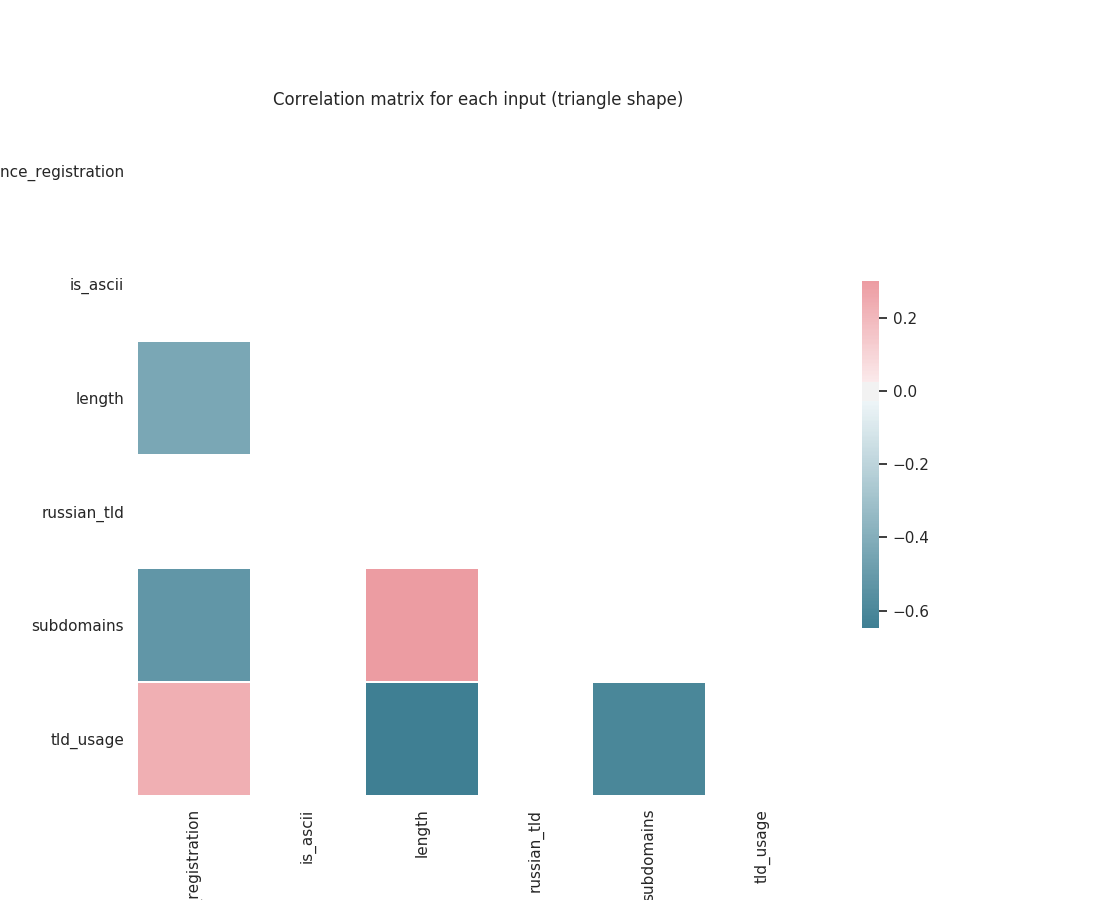
\includegraphics[width=\linewidth]{correlation_matrix}
  \caption{Correlation matrix}
  \label{correlation-matrix}
\end{figure}

\subsection{Classifiers}
During our first steps in the project, we tried to behave like a classifier,
asking ourselves how should we proceed to classify a URL between two states :
safe or unsafe. As a human we can easily observe independant characteristics of
an object. For a URL, we observed the length and the number of subdomains at
first glance. These are independant characteristics that suggests a correlation:
the more subdomains a URL have, the more it is long. As a human we can treat
length characteristic as a conditional variable depending on subdomains, in
mathematics, such reasoning is attributed to Thomas Bayes (and its Bayes'
theorem). We found during our researches that we can use this theorem to
classify data, it is known as the naive bayes classifier. It's a linear
classifier based on applying Bayes' theorem with strong (naive) independance
between observed characteristics (features). As we continued ou researches, we
found that this kind of frequentialist approach (or Bayesian inferential
approach) was not the only one and we quickly felt overwhelmed by all the common
techniques for supervised classification problems. We discovered SVMs (%
Support-Vector Machines) (another linear classifier), kNN technique (k-Nearest
Neighbors algorithm), NN (Neural Network and derivates), decision trees and
its agglomeration in random forets and some more. With only length and subdomain
count as features, we were able to represent our training and testing datasets
on a 2D graph, what we did. The figure \ref{classifiers-list} represents the
different classifiers we tried over our dataset. The blue points corresponds to
the unsafe URLs and the red ones to the safe ones. The semi-transparent points
are the testing points and the plain ones, the training ones. The high accuracy
is due to the fact that we use approximately 95\% of 1-subdomain safe URLs: we
can easily spot the red cluster aligned on the bottom line for one subdomain.
Note that subdomains go from 1 to 3. However, it's interesting to visualize how
these classifiers are splitting the 2D space. Visualization turned out to be
very handy to detect problems with our datasets and to select the most
appropriate features.

\begin{figure}[!t]
  \centering
  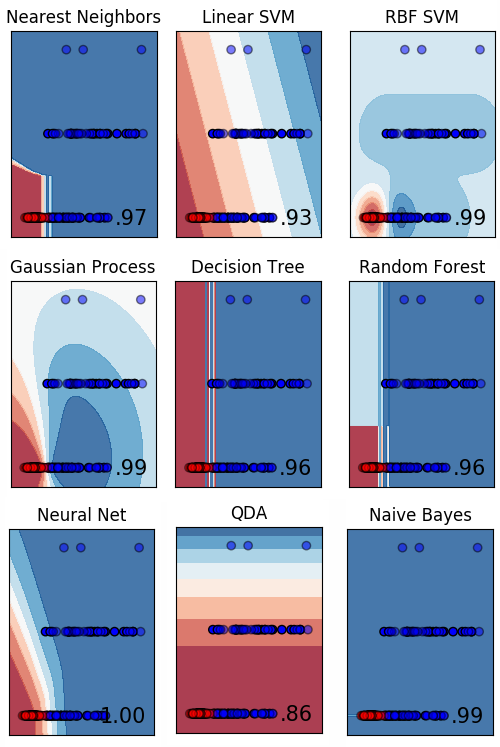
\includegraphics[width=\linewidth]{classifiers-list}
  \caption{Classifiers}
  \label{classifiers-list}
\end{figure}

\section{Datasets}
Over the time, we built two datasets for safe and unsafe URLs from various
sources. Those datasets are dynamic and are updated whenever our sources are
updating theirs. We support caching as well. \\

Unsafe URLs sources :
\begin{itemize}
  \item PhishTank project api \cite{phishtank}
  \item CyberCrime database \cite{cybercrime}
  \item University of New Brunswick \cite{unb-website} \cite{unb-article}
\end{itemize}
Safe URLs sources :
\begin{itemize}
  \item Alexa top 1 million websites \cite{alexa-top-1m}
  \item University of New Brunswick \cite{unb-website} \cite{unb-article}
\end{itemize}

\section{Our performance}
The following results were obtained from a set of 1337 safe URLs and 1337 unsafe
URLs. 60\% of those have been used to train the models and the 40\% remaining to
test the models.

\begin{table}[]
  \centering
  \begin{tabular}{|l|l|l|}
  \hline
    Classifier        & Accuracy & Parameters \\ \hline
    Linear SVM        & 0.928    & penalty = 0.025\\ \hline
    RBF SVM           & 0.953    & kernel coef = 2, penalty = 1\\ \hline
    Nearest neighbors & 0.919    & 3 nearest neighbors\\ \hline
    Decision tree     & 0.984    & m depth = 5\\ \hline
    Random forest     & 0.974    & m depth = 5, n estimators = 1, f max = 1\\ \hline
    AdaBoost          & 0.984    & \\ \hline
    Naive Bayes       & 0.983    & \\ \hline
    LDA               & 0.830    & \\ \hline
    QDA               & 0.981    & \\ \hline
    Gaussian Process  & 0.983    & kernel = 1.0 * RBF(1.0)\\ \hline
    Neural Network    & 0.941    & \\ \hline
  \end{tabular}
\end{table}

The timings (with data reading / writing steps) :
\begin{itemize}
  \item 579,09s user
  \item 285,23s system
  \item 46\% cpu
  \item 30:42,48 total
\end{itemize}

\section{Conclusion and future work}
We enjoyed the project as we worked on new topics and discovered some cool
things around multivariate statistics, data mining and analysis, data
visualization, classification and prediction. Our strongest correlation will
remain the one linking the length and the number of subdomains of a URL. \\
One big improvment step would be to build I/O to the program in order to allow
new URLs. We could then proceeed to unsupervised learning. We could connect this
I/O system to a fancy front-end in order for people to test their URLs while
increasing the accuracy of the model but we can also link it to mail server in
order to classify and prevent malicious mails, or any live stream of data that
would help increasing the model relevance. \\
Another good step would be to dynamically test features (may it be bucket or
split testing) in order to be able to choose them more specifically and to
reveal possible local maxima. \\

Here are some pertinent future feature ideas:
\begin{itemize}
  \item Pagerank computation (api limitations)
  \item Prohibited statuses in whois infos (registrant takes care of its domain)
  \item Count redirections (is website stable ?)
  \item Homoglyphs and the internation domain name (IDN) homograph attack
  \item Typosquatting (can compare Hamming distance to safe brand names)
\end{itemize}

%\section{References}
\bibliographystyle{abbrv}
\bibliography{report}

\end{document}
